% Drawing 154/07-18 -- folder 154, batch 07, archive page 126 (PDF page 127).
% Transcription: en haut, une bande : une droite vert clair entre deux droites brunes, coupée de croisements orange ; les segments de la droite supérieure sont marqués $p'$, $q'$, $s'$, $u'$, $v'$, $w'$, $y'$, $z'$, ceux de l'inférieure $p$, $q$, $r$, $t$, $u$, $w$, $x$, $z$, avec des barres noires sur certains croisements. À droite, un cercle au crayon traversé de droites orange, aux extrémités marquées de barres bleues ; des morceaux de graphe vert (en H, en Y) ; un heptagone bleu avec des cordes orange et une étoile verte au centre. En bas, des étoiles au crayon avec des flèches, une fleur de pétales hachurés et un grand « $2$ » ; un petit peigne orange
% Kind: page of sketches: strip with lettered segments, disk, green graphs, heptagon. Method 2 (schematic redraw from the facsimile). Status: partial.
% Notes: Strip: three slightly arched lines (brown, light green, brown), five groups of orange strokes crossing them, four short black bars at the first and fourth groups, the letters of the upper and of the lower line as the transcription reads them. Circle: pencil rim, a vertical and a horizontal orange spindle and two diagonals, a short blue bar at four ends. Green: an H with three points and a Y hanging from it, a piece shaped like two Y's joined by a dark stroke, a small Y. Heptagon: blue outline, seven green rays from an inner point, of which four run on beyond the outline; the orange chords inside it are left out. Bottom: a pencil star with two arrows, a flower of six petals with a point, the figure 2, and the orange comb with a dark bar on its first tooth gap. Everything is placed from a page view and simplified; the small marks x, 1, 2, 3 on the strip and the pencil hatching of the petals are left out. Redrawn 2026-11-12 (issue 128): to check again. 2026-11-14, Claude Opus 5.5, overlay check (issue 147): rasterised from its own coordinates over the 400 dpi colour scan (402 ppi native) on a unit grid; not compiled (no TeX in the session). The strip with its crossings and letters, the green H and Y pieces, the pencil star, the arrows, the 2 and the comb lie on their ink to within about 1 to 1.5 units; the redraw is unchanged. Still partial for the reasons given above: inside the pencil circle the orange strands are drawn as two spindles and two diagonals where the page has curved strands of its own; the six petals of the flower are drawn as two crossed ellipses, unhatched; the orange chords of the heptagon are not drawn and its green rays are placed approximately; faint pencil circles behind the figures are not drawn.
% Coordinates: 1 unit = 1 mm = 1/100 of the crop width (bbox in page fractions: [0.16, 0.19, 0.96, 0.52]).
% Redrawn by Claude (claude-fable-5-2), issue #128, 2026-11-12; not checked by a human; not compiled (no TeX in the session).
% Checked by Claude (claude-opus-5-5) 2026-11-14 (issue #147): overlaid on the 400 dpi colour facsimile; not compiled (no TeX in the session). Not checked by a human. Status: partial.
% Rights: reproduces part of the work -- behind RENDER_TRANSCRIPTS, never published by itself.
\documentclass[tikz,border=3pt]{standalone}
\usepackage{amsmath,amssymb}
\usetikzlibrary{patterns,arrows.meta}
\tikzset{Or/.style={orange!90!black}, Lg/.style={green!60!black!70}, Dg/.style={green!45!black}, Br/.style={brown!80!black}, Bl/.style={blue!70!black}, pencil/.style={black!45}, struck/.style={black!35}, mpt/.style={circle,draw,inner sep=1.3pt}, pt/.style={circle,fill,inner sep=0.9pt}, opt/.style={circle,draw,fill=white,inner sep=1.1pt}}
\begin{document}
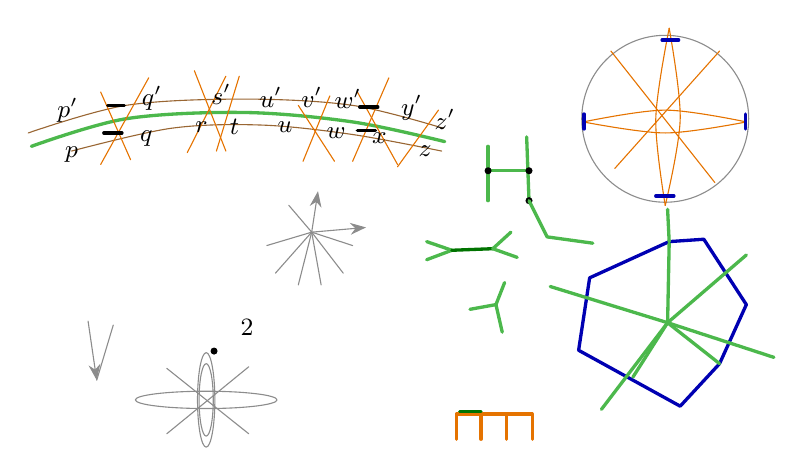
\begin{tikzpicture}[x=1mm,y=1mm,line cap=round,line join=round,font=\scriptsize]
\draw[Br] plot[smooth, tension=0.55] coordinates {(1.2,-15.1) (13.6,-11.6) (28.6,-10.8) (42.4,-11.6) (53.9,-14.5)};
\draw[Lg,very thick] plot[smooth, tension=0.55] coordinates {(1.6,-16.8) (13.6,-13.3) (28.6,-12.5) (42.4,-13.7) (54.1,-16.2)};
\draw[Br] plot[smooth, tension=0.55] coordinates {(6.7,-17.4) (19.4,-14.5) (30.9,-14.1) (42.4,-15.3) (53.7,-17.4)};
\draw[Or] (10.4,-9.9) -- (14.2,-18.5);
\draw[Or] (16.5,-8.1) -- (10.4,-19.1);
\draw[Or] (22.3,-7.2) -- (26.3,-17.4);
\draw[Or] (26.3,-7.9) -- (21.4,-17.6);
\draw[Or] (28,-7.9) -- (25.1,-17.4);
\draw[Or] (35.5,-11.6) -- (40.1,-18.7);
\draw[Or] (39.5,-10.4) -- (36.1,-18.7);
\draw[Or] (43,-9.9) -- (48.1,-19.1);
\draw[Or] (47,-8.1) -- (42.4,-18.7);
\draw[Or] (53.3,-12.2) -- (48.1,-19.4);
\draw[very thick] (11.3,-11.6) -- (13.4,-11.6);
\draw[very thick] (10.8,-15.1) -- (13.1,-15.1);
\draw[very thick] (43.3,-11.8) -- (45.6,-11.8);
\draw[very thick] (43,-14.8) -- (45.3,-14.8);
\node[inner sep=1pt] at (6.2,-12.2) {\small $p'$};
\node[inner sep=1pt] at (16.9,-10.7) {\small $q'$};
\node[inner sep=1pt] at (25.7,-10.2) {\small $s'$};
\node[inner sep=1pt] at (32,-10.6) {\small $u'$};
\node[inner sep=1pt] at (37.2,-10.6) {\small $v'$};
\node[inner sep=1pt] at (41.8,-10.8) {\small $w'$};
\node[inner sep=1pt] at (49.9,-11.9) {\small $y'$};
\node[inner sep=1pt] at (54.1,-13.4) {\small $z'$};
\node[inner sep=1pt] at (6.7,-17.8) {\small $p$};
\node[inner sep=1pt] at (16.2,-15.8) {\small $q$};
\node[inner sep=1pt] at (23.2,-14.3) {\small $r$};
\node[inner sep=1pt] at (27.4,-14.3) {\small $t$};
\node[inner sep=1pt] at (33.8,-14.3) {\small $u$};
\node[inner sep=1pt] at (40.3,-15.1) {\small $w$};
\node[inner sep=1pt] at (45.8,-15.8) {\small $x$};
\node[inner sep=1pt] at (51.6,-17.4) {\small $z$};
\draw[pencil] (82.1,-13.3) circle[radius=10.6];
\draw[Or] plot[smooth, tension=0.55] coordinates {(82.6,-1.8) (80.9,-13.3) (82.1,-24.3)};
\draw[Or] plot[smooth, tension=0.55] coordinates {(82.6,-1.8) (84,-13.3) (82.1,-24.3)};
\draw[Or] plot[smooth, tension=0.55] coordinates {(71.7,-13.7) (82.1,-12.2) (92.4,-13.7)};
\draw[Or] plot[smooth, tension=0.55] coordinates {(71.7,-13.7) (82.1,-15.1) (92.4,-13.7)};
\draw[Or] (75.2,-4.7) -- (88.4,-21.4);
\draw[Or] (89,-4.7) -- (75.7,-19.6);
\draw[Bl,very thick] (81.7,-3.3) -- (83.8,-3.3);
\draw[Bl,very thick] (80.9,-23.1) -- (83.2,-23.1);
\draw[Bl,very thick] (71.8,-12.7) -- (71.8,-14.6);
\draw[Bl,very thick] (92.3,-12.7) -- (92.3,-14.6);
\draw[Lg,very thick] (59.6,-16.8) -- (59.6,-23.7);
\draw[Lg,very thick] (64.5,-15.6) -- (64.8,-23.7);
\draw[Lg,very thick] (59.6,-19.9) -- (64.8,-19.9);
\node[pt] at (59.6,-19.9) {};
\node[pt] at (64.8,-19.9) {};
\node[pt] at (64.8,-23.7) {};
\draw[Lg,very thick] (64.8,-23.7) -- (67.1,-28.3) -- (72.9,-29.1);
\draw[Lg,very thick] (51.8,-31.2) -- (55,-30);
\draw[Lg,very thick] (51.8,-28.9) -- (55,-30);
\draw[Dg,very thick] (55,-30) -- (60.2,-29.8);
\draw[Lg,very thick] (60.2,-29.8) -- (63.3,-30.9);
\draw[Lg,very thick] (60.2,-29.8) -- (62.5,-27.7);
\draw[Lg,very thick] (57.3,-37.5) -- (60.6,-36.9);
\draw[Lg,very thick] (60.6,-36.9) -- (61.7,-34.1);
\draw[Lg,very thick] (60.6,-36.9) -- (61.4,-40.4);
\draw[Bl,very thick] (82.6,-28.9) -- (87,-28.6) -- (92.4,-36.9) -- (89,-44.4) -- (84,-49.8) -- (71.1,-42.7) -- (72.5,-33.5) -- cycle;
\draw[Lg,very thick] (82.4,-39.2) -- (82.6,-29.1);
\draw[Lg,very thick] (82.4,-39.2) -- (92.4,-30.6);
\draw[Lg,very thick] (82.4,-39.2) -- (95.9,-43.6);
\draw[Lg,very thick] (82.4,-39.2) -- (74,-50.2);
\draw[Lg,very thick] (82.4,-39.2) -- (67.5,-34.6);
\draw[Lg,very thick] (82.4,-39.2) -- (78,-46.1);
\draw[Lg,very thick] (82.4,-39.2) -- (89,-44.4);
\draw[Lg,very thick] (82.6,-28.9) -- (82.4,-24.8);
\draw[pencil] (37.2,-27.7) -- (31.5,-29.4);
\draw[pencil] (37.2,-27.7) -- (32.6,-32.9);
\draw[pencil] (37.2,-27.7) -- (35.5,-34.4);
\draw[pencil] (37.2,-27.7) -- (38.4,-34.4);
\draw[pencil] (37.2,-27.7) -- (41.2,-32.9);
\draw[pencil] (37.2,-27.7) -- (42.4,-29.4);
\draw[pencil] (37.2,-27.7) -- (34.3,-24.3);
\draw[pencil,-{Stealth[length=2mm]}] (37.2,-27.7) -- (38,-22.5);
\draw[pencil,-{Stealth[length=2mm]}] (37.2,-27.7) -- (44.1,-27.1);
\draw[pencil] (23.8,-49) ellipse[x radius=1.1, y radius=6];
\draw[pencil] (23.8,-49) ellipse[x radius=9, y radius=1.1];
\draw[pencil] (23.8,-49) ellipse[x radius=0.9, y radius=4.6];
\draw[pencil] (18.8,-45) -- (29.2,-53.3);
\draw[pencil] (29.2,-44.8) -- (18.8,-53.3);
\node[pt] at (24.8,-42.8) {};
\node[inner sep=1pt] at (29,-39.8) {\small $2$};
\draw[pencil,-{Stealth[length=2mm]}] (8.8,-39) -- (9.9,-46.5);
\draw[pencil] (12,-39.5) -- (9.9,-46.5);
\draw[Or,very thick] (55.6,-54) -- (55.6,-50.8) -- (65.2,-50.8) -- (65.2,-54);
\draw[Or,very thick] (58.7,-50.8) -- (58.7,-54);
\draw[Or,very thick] (61.9,-50.8) -- (61.9,-54);
\draw[Dg,very thick] (56,-50.5) -- (58.7,-50.5);
\end{tikzpicture}
\end{document}
